\begin{center}

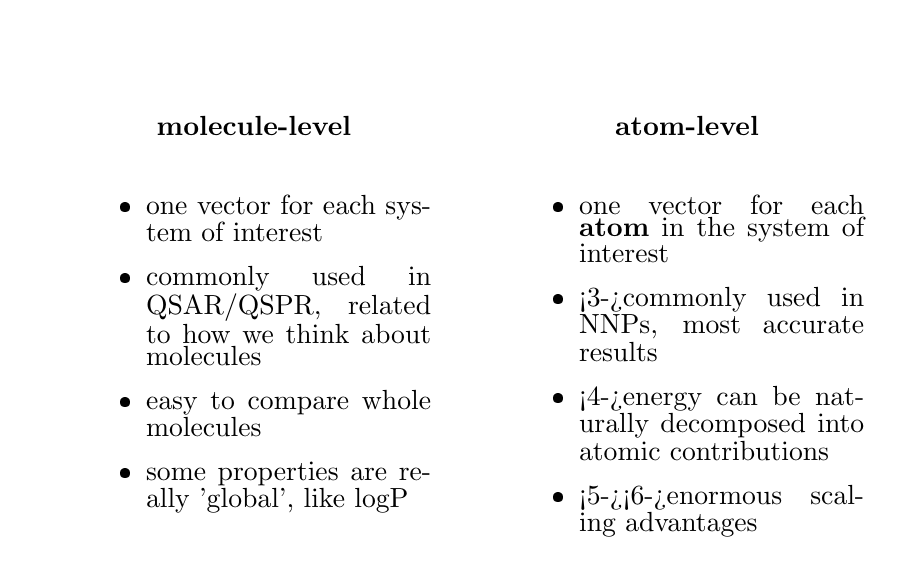
\begin{tikzpicture}[x=1cm,y=1cm]
\tikzstyle{line} = [draw, -latex', very thick]
\draw[use as bounding box, anchor = north west,draw=none] (-1,-1) rectangle (5.5+4.5,3.25+2.25);
\clip (-1,-1) rectangle (10,5.5);
\linespread{0.5}
%\path [draw,very thick,->] (cxe) edge node[above] {cost}  (corig);
\visible<1->{\node [text badly centered,black,text width = 4.5cm,anchor=north west] (lab13) at (-0.5,4.5) {\textbf{molecule-level}};}

\visible<1->{\node [align = flush left,black,text width = 3.25cm,anchor=north west] (lab13) at (-0.5,3.5) {
		\begin{minipage}{4.5cm}
		\begin{itemize}
		\item one vector for each system of interest
		\item commonly used in QSAR/QSPR, related to how we think about molecules
		\item easy to compare whole molecules
		\item some properties are really 'global', like logP
		\end{itemize}
		\end{minipage}};}
\visible<2->{\node [text badly centered,black,text width = 4.5cm,anchor=north west] (lab13) at (5,4.5) {\textbf{atom-level}};}
\visible<2->{\node [align = flush left,black,text width = 3.25cm,anchor=north west] (lab13) at (5,3.5) {
		\begin{minipage}{4.5cm}
		\begin{itemize}
		\item one vector for each \textbf{atom} in the system of interest
		\item \visible<3->{commonly used in NNPs, most accurate results}
		\item \visible<4->{energy can be naturally decomposed into atomic contributions}
		\item \visible<5->{\only<6->{\color{red}}enormous scaling advantages}
		\end{itemize}
		\end{minipage}};}

\end{tikzpicture}

\end{center}
